The median \ac{os} in the entire population treated with \ac{cdk46i} was 46 months (95\% CI 39.4–55.6). Median \ac{pfs} was 20.1 months (95\% CI 18.3–24.2). Following this, we compared Palbociclib and ribociclib only as first-line treatments. We found that regarding \ac{os}, there is no significant difference between the two, but ribociclib is significantly better in terms of \ac{pfs} (\textit{P} value $\le$ 0.001) (Figure \ref{fig:interest}). Additionally, we compared the same \ac{cdk46i} with letrozole as a combination only (PAL-LT and RIB-LT). Regarding this scenario, we found out that both were similar in terms of \ac{os} and \ac{pfs}.


\begin{figure}[ht]
  \caption{Survival curves for Palbociclib and Ribociclib (1st line) - \ac{pfs} and \ac{os}}\label{fig:interest} 
  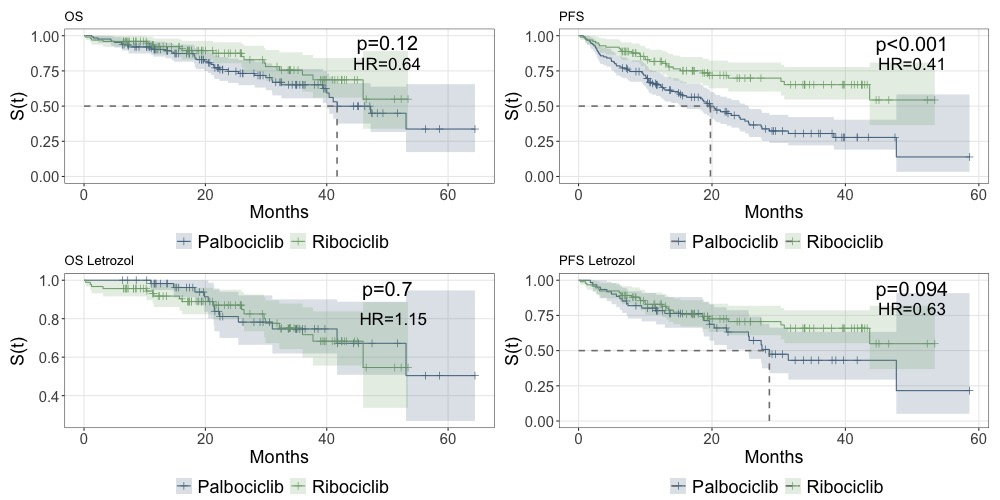
\includegraphics[scale=0.45]{figures/interest_curve_both.jpeg}%

\end{figure}


We then compared both with a cox regression, where \ac{os} shows no significant difference between palbociclib and ribociclib when adjusted to the stage, visceral metastases, age, treatment line, combination and \ac{ecog}. The proportional hazards' assumption was confirmed with \textit{P} values all over 0.10.
\begin{table}[ht]
  \centering
  \caption{Cox Regression with palbociclib and Ribociclib - \ac{pfs} and \ac{os}}\label{tab:cox} 
  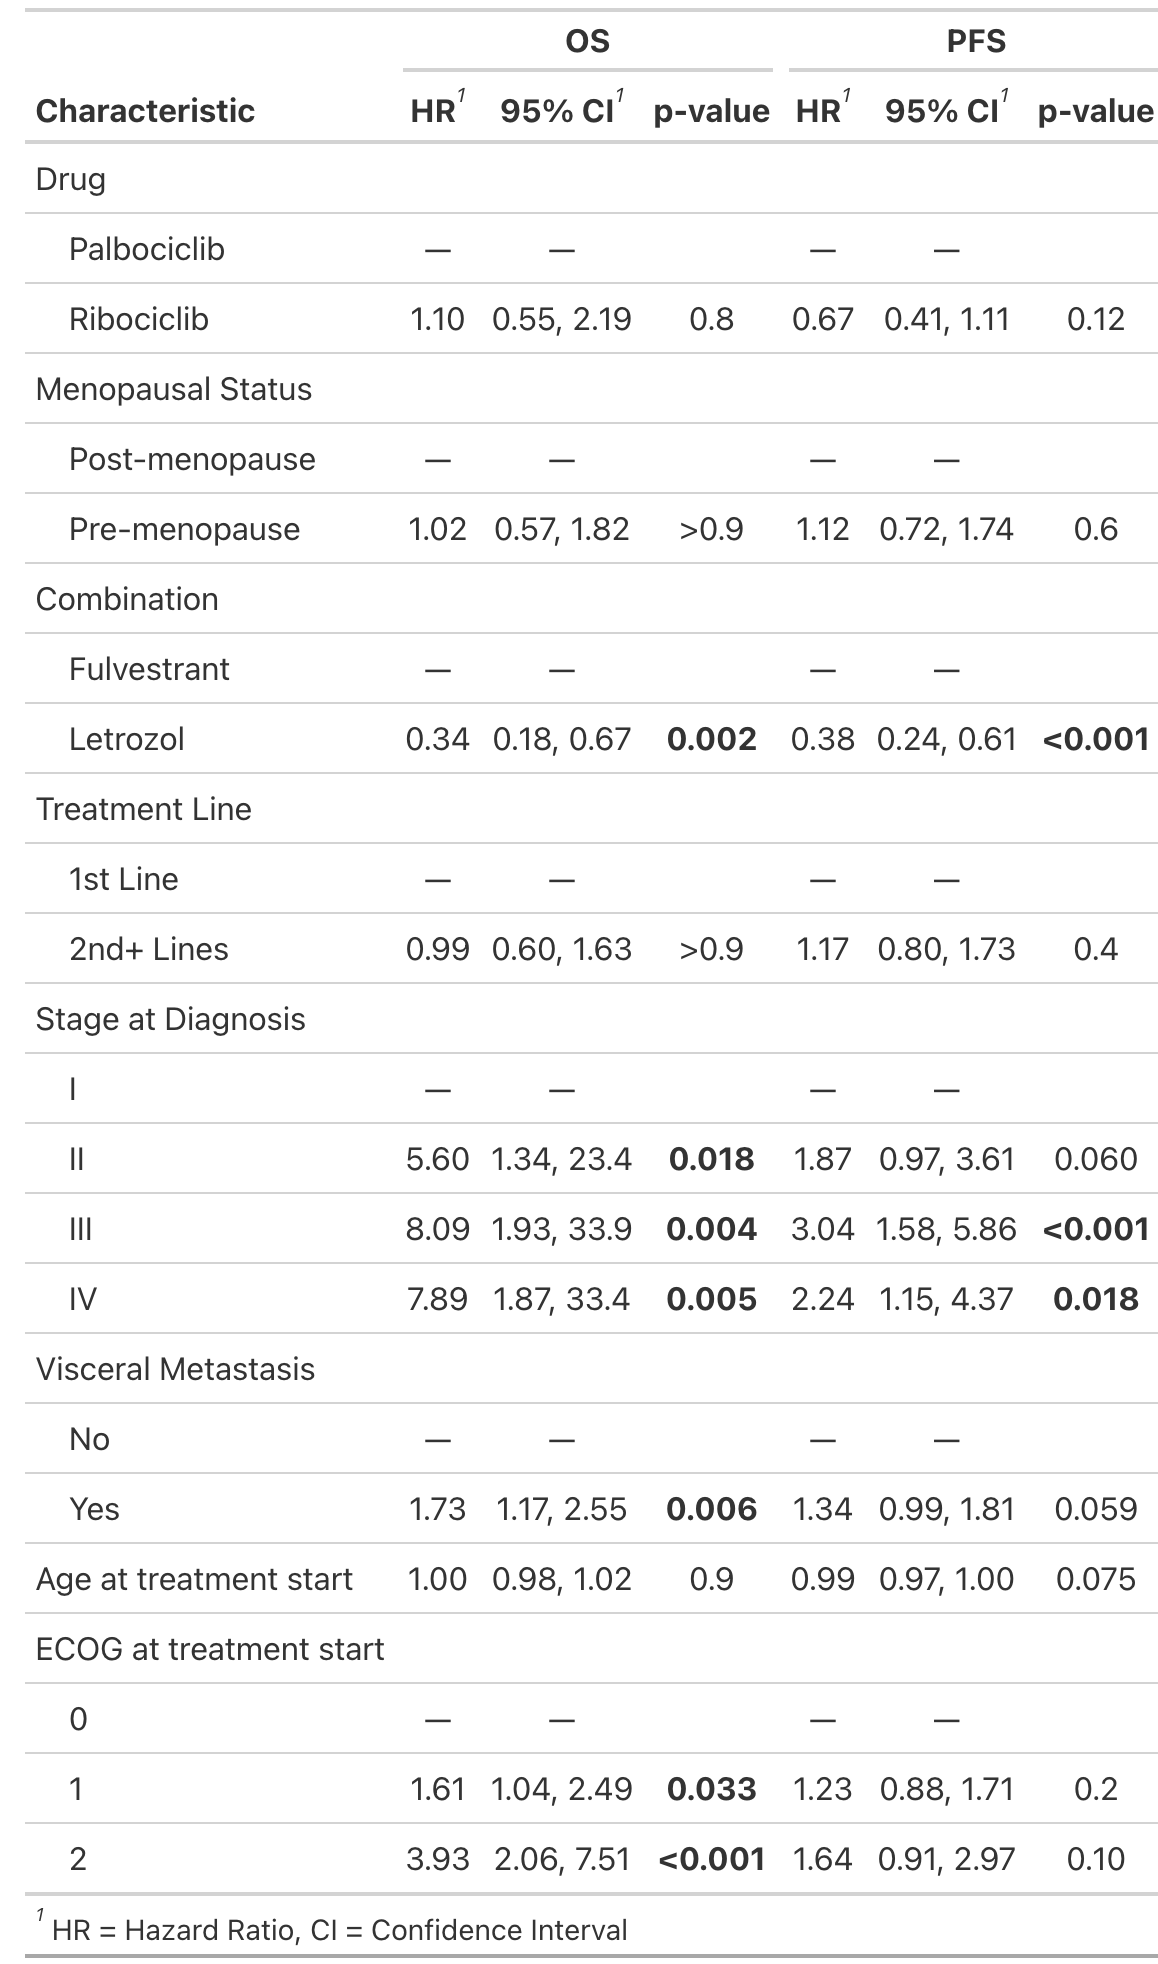
\includegraphics[scale=0.20]{figures/cox_both.png}%

\end{table}

When comparing \ac{et} with \ac{cdk46i} as first-line treatment (figure \ref{fig:grouped}). For this study we only compared patients with bone only metastasis. When comparing both \ac{cdk46i} combined with Fulvestrant or letrozole, we see that  Ribociclib (RIB+LT/FUL) is significantly better for \ac{pfs} (\textit{P} value $\le$ 0.001 \ac{hr}=0.21) but not \ac{os}. For Palbociclib as the first line with Fulvestrant or letrozole (PAL+LT/FUL), we see that there is no significant difference in terms of \ac{pfs} and \ac{os} (\textit{P}=0.57 and 0.51). We also applied the same analysis but comparing only the letrozole combination with letrozole alone (PAL-LT/RIB-LT vs LT). We found that both ribociclib and palbociclib are significantly better in terms of \ac{pfs} (\ac{hr} 0.65 for palbociclib and 0.27 for ribociclib) but not \ac{os}.
\begin{figure}[ht]
  \centering

  \caption{Survival curves (\ac{os} and \ac{pfs}) comparing \ac{et} to \ac{cdk46i} combined with fulvestrant or letrozole as 1st line. First row is \ac{cdk46i} combined fulvestrant or letrozole vs fulvestrant or letrozole. Second row is \ac{cdk46i} combined with letrozole vs letrozole alone. \textit{P} values shown as pairwise vs. ET. }\label{fig:grouped} 
  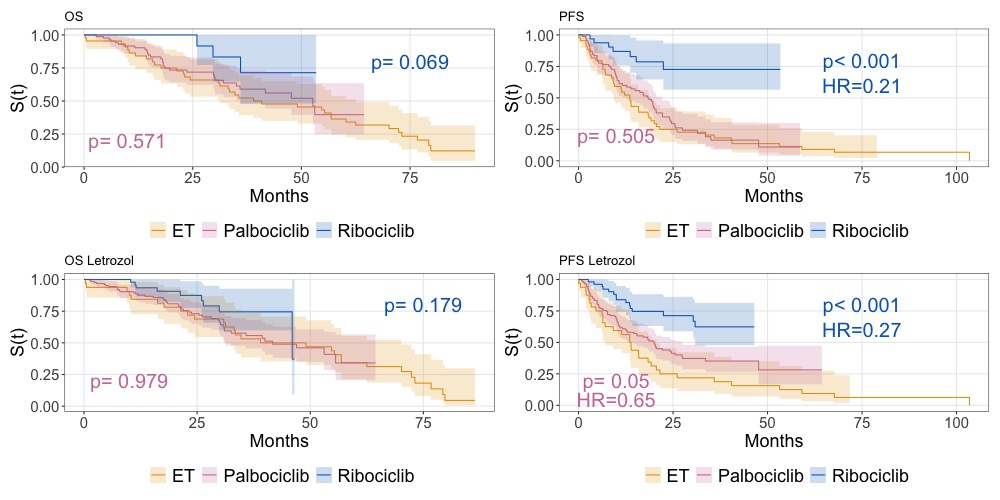
\includegraphics[scale=0.42]{figures/grouped_curve_both.jpeg}%

\end{figure}

When comparing palbociclib and ribociclib adjusted for \ac{ate} weights, we found a different scenario from previous assessments. There is a significant difference between the two in terms of \ac{os} (figure \ref{fig:propensity}). The weights were calculated as stated in the methods section.


\begin{figure}[ht]
  \centering

  \caption{Comparison of palbociclib and ribociclib survival curves adjusted for propensity scores}\label{fig:propensity} 
  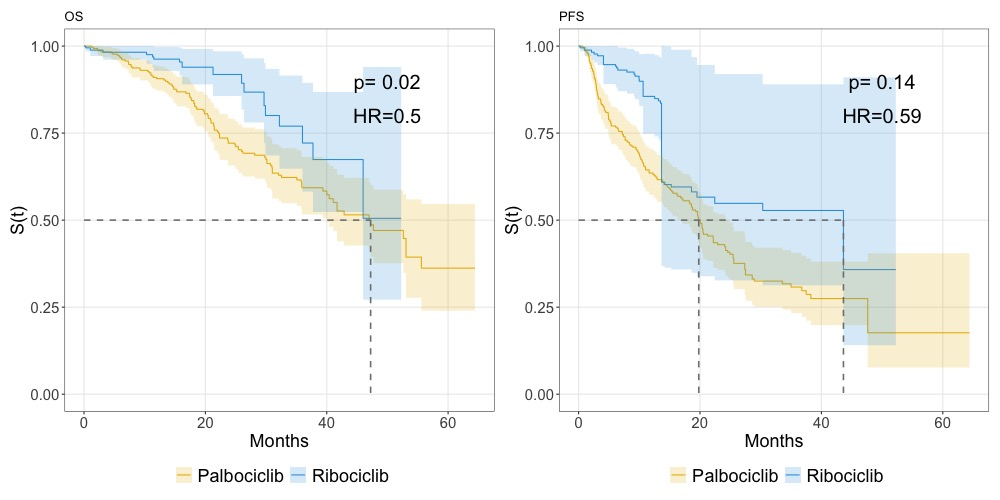
\includegraphics[scale=0.42]{figures/propensity_score_both.jpeg}%

\end{figure}

The Cox regression adjusted for the variables and with the weights applied to render an \ac{hr}=0.55 [95\% CI 0.28-1.09;\textit{P}=0.086] for \ac{os}. The \ac{hr}for \ac{pfs} is 0.56 [95\% CI 0.32-1;\textit{P}=0.05].